\subsection{线性不相交扩张}

在整个这一节中，\(\Omega\) 表示域 K 的一个扩张。

设 A 和 B 是 \(\Omega\) 的两个 K-子代数。存在一个代数同态 \(\varphi: \mathbf{A} \otimes_{\mathbf{K}} \mathbf{B} \to \Omega\) ，它把 \(x \otimes y\) 映到 \(xy\) 。\(\varphi\) 的像是 \(\Omega\) 中由 \(\mathbf{A} \cup \mathbf{B}\) 生成的子环 C。此外，根据 II，第 256 页，若 \((b_{\mu})\) 是 B 在 K 上的一组基，而 \((a_{\lambda})\) 是 A 在 K 上的一组基，则 C 与形如 \(\sum_{\mu} \alpha_{\mu} b_{\mu}\) （其中 \(\alpha_{\mu} \in \mathbf{A}\) ）的线性组合的集合一致，也是所有形如 \(\sum_{\lambda} \beta_{\lambda} a_{\lambda}\) （其中 \(\beta_{\lambda} \in \mathbf{B}\) ）的集合，以及所有形如 \(\sum_{\lambda, \mu} \gamma_{\lambda \mu} a_{\lambda} b_{\mu}\) （其中 \(\gamma_{\lambda \mu} \in \mathbf{K}\) ）的集合。

我们将称A和B在K上是线性不相交的，如果 \(\varphi\) 是 \(A \otimes_{K} B\) 到 C 上的同构。于是我们有 \(A \cap B = K\) ；B（相应地，A）的每个关于K的自由子集于是关于A（相应地，B）是自由的；反之，为使A和B在K上线性不相交，只需存在B在K上的一个基（例如）关于A是自由的（II，第256页及III，第469页）。

特别地，考虑 A 和 B 是 \(\Omega\) 的子扩张的情形。

命题5. --- 设E和F是包含在Ω中的K的两个扩张。

\begin{enumerate}
\def\labelenumi{\alph{enumi})}
\item
  如果 F 在 K 上具有有限次数，则 \(\Omega\) 中由 \(E \cup F\) 生成的子环是一个域，它与 \(\mathrm{E}(\mathrm{F})\) 一致，且 \(\mathrm{E}(\mathrm{F})\) 在 E 上的次数是有限的；我们有 \([\mathrm{E}(\mathrm{F}):\mathrm{E}] \leqslant [\mathrm{F}:\mathrm{K}]\) ，其中等号成立当且仅当 E 与 F 在 K 上线性不相交。在这种情况下 \(\mathrm{E}(\mathrm{F})\) 与 \(E \otimes_{K} F\) 是 E-同构的。
\item
  若E在K上具有有限次数，则 \(\mathrm{E}(\mathrm{F})=\mathrm{K}(\mathrm{E}\cup\mathrm{F})\) 在K上是有限次的。我们有 \([\mathrm{K}(\mathrm{E}\cup\mathrm{F}):\mathrm{K}]\leqslant[\mathrm{E}:\mathrm{K}][\mathrm{F}:\mathrm{K}]\) ，当且仅当E和F在K上线性不相交时等号成立。
\end{enumerate}

设 C 为 \(\Omega\) 中由 \(E \cup F\) 生成的子环；如果 \((b_j)_{1 \leq j \leq n}\) 是 \(F\) 在 \(K\) 上的一组基，则 \(C\) 是 \(\Omega\) 的由诸 \(b_j\) 生成的 E-向量子空间，因此 \(C\) 是一个有限秩代数，其秩 \(\leq n\) ，且位于 \(E\) 上；由于环 \(C\) 包含于一个域中，它是整环，因此由命题 1 的推论（V，第 10 页）可知它是一个域，从而 \(C = E(F)\) 且 \([E(F):E] \leq [F:K]\) 。关系式 \([E(F):E] = [F:K]\) 意味着诸 \(b_j\) 在 \(E\) 上线性无关，因此 \(E\) 与 \(F\) 在 \(K\) 上线性不相交；这证明了命题的第 \(a)\) 部分。第 \(b)\) 部分现在立即由 \([E(F):K] = [E(F):E][E:K]\) 这一事实得出。

设 E 和 F 是包含在 \(\Omega\) 中的 K 的扩张。若 E 和 F 在 K 上具有无限次数，则子环 \(C = K[E \cup F]\) 不一定是域 \(^{1}\) ；然而此时 C 的分式域恰好与 \(K(E \cup F)\) 一致。更一般地，设 A 是 E 的一个子环，使得 E 是 A 的分式域，并设 B 是 F 的一个子环，使得 F 是 B 的分式域；那么若 C 是 \(\Omega\) 中由 \(A \cup B\) 生成的子环，则 \(K(E \cup F)\) 与 C 的分式域一致，因为后一个域是 \(\Omega\) 中包含 C 的最小子域，且它包含 E 和 F。此外：

命题6. --- 设E和F是包含在Ω中的K的两个扩张，且A和B是Ω上K的两个子代数，使得E是A的分式域，F是B的分式域。则E和F在K上线性不相交当且仅当A和B在K上线性不相交。

该条件是显然必要的。反之，若A和B在K上线性不相交，则A和F也如此，因为若 \(\Omega\) 中的一族元素关于 B 是自由的，则它关于 B 的分式域 F 也是自由的（II，第 315 页，推论 1 及第 316 页，推论 3）；现在同样的论证表明 E 与 F 在 K 上是线性不相交的。

\(^{1}\) 只需考虑例如这样的情形：\(\Omega\) 是两个不定元 X 和 Y 上的有理分式域 \(\mathbf{K}(\mathbf{X},\mathbf{Y})\) ，且 \(\mathbf{E}=\mathbf{K}(\mathbf{X}),\mathbf{F}=\mathbf{K}(\mathbf{Y})\) 。

命题 7. --- 设 E 和 F 是包含在 Ω 中的 K 的两个扩张；若 E 和 F 在 K 上线性不相交，则 E 的每个子扩张和 F 的每个子扩张都在 K 上线性不相交。反之，若对于 E 和 F 的每一对有限生成子扩张 E'、F'（分别属于 E 和 F），E' 和 F' 都在 K 上线性不相交，则 E 和 F 在 K 上线性不相交。

因为 E 和 F 在 K 上线性不相交的条件可以这样表述：若 \((a_{\alpha})\) 是 E 中的一个自由族， \((b_{\beta})\) 是 F 中的一个自由族，则关系 \(\sum_{\alpha,\beta}\lambda_{\alpha\beta}a_{\alpha}b_{\beta}=0\) ，其中 \(\lambda_{\alpha\beta}\in K\) 蕴含 \(\lambda_{\alpha\beta}=0\) 对每一对下标成立。但若该条件对每一对有限自由族成立，则它对每一对自由族也成立。

因此，我们可以直观地说，线性不相交性是一个“有限特征”的性质。

命题 8. --- 设 E、F、G 是包含在 \(\Omega\) 中的域 K 的三个扩张，使得 \(F \subset G\) 。要使 E 和 G 在 K 上线性不相交，当且仅当 E 和 F 在 K 上线性不相交，且 E(F) 和 G 在 F 上线性不相交。

\pandocbounded{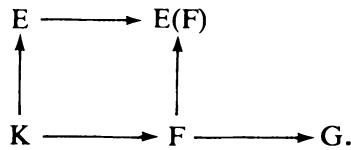
\includegraphics[keepaspectratio]{images/part001_e5f97af6.jpg}}\\
图 2.

条件必要性：假设 E 和 G 在 K 上线性不相交。那么 E 和 F 也如此（命题 7）；另一方面，若 B 是 E 在 K 上的一组基，则它也是代数 F{[}E{]} 在 F 上的一组基；由于由假设 B 在 G 上自由，F{[}E{]} 和 G 在 F 上线性不相交，且由命题 6，E(F) = F(E) 和 G 也如此。

条件充分性：用同样的记号，该条件蕴含 B 在 F 上自由，因此它是 F{[}E{]} 在 F 上的一组基；由于由假设 F{[}E{]} 和 G 在 F 上线性不相交，B 在 G 上自由，这表明 E 和 G 在 K 上线性不相交。

